\documentclass[12pt]{article}
\usepackage[utf8]{inputenc}
\usepackage[usenames]{color}
\usepackage[margin=1in]{geometry} 
\usepackage{amsmath,amsthm,amssymb,graphicx,mathtools,tikz,hyperref, pgfplots, listings, pdfpages}
\usetikzlibrary{positioning}
\newcommand{\n}{\mathbb{N}}
\newcommand{\z}{\mathbb{Z}}
\newcommand{\q}{\mathbb{Q}}
\newcommand{\cx}{\mathbb{C}}
\newcommand{\real}{\mathbb{R}}
\newcommand{\field}{\mathbb{F}}
\newcommand{\ita}[1]{\textit{#1}}
\newcommand{\com}[2]{#1\backslash#2}
\newcommand{\oneton}{\{1,2,3,...,n\}}
\newcommand\idea[1]{\begin{gather*}#1\end{gather*}}
\newcommand\ef{\ita{f} }
\newcommand\eff{\ita{f}}
\newcommand\proofs[1]{\begin{proof}#1\end{proof}}
\newcommand\inv[1]{#1^{-1}}
\newcommand\setb[1]{\{#1\}}
\newcommand\en{\ita{n }}
\newcommand{\vbrack}[1]{\langle #1\rangle}


\newenvironment{theorem}[2][Teorema]{\begin{trivlist}
\item[\hskip \labelsep {\bfseries #1}\hskip \labelsep {\bfseries #2.}]}{\end{trivlist}}
\newenvironment{lemma}[2][Lema]{\begin{trivlist}
\item[\hskip \labelsep {\bfseries #1}\hskip \labelsep {\bfseries #2.}]}{\end{trivlist}}
\newenvironment{exercise}[2][Ejercicio]{\begin{trivlist}
\item[\hskip \labelsep {\bfseries #1}\hskip \labelsep {\bfseries #2.}]}{\end{trivlist}}
\newenvironment{reflection}[2][Reflexión]{\begin{trivlist}
\item[\hskip \labelsep {\bfseries #1}\hskip \labelsep {\bfseries #2.}]}{\end{trivlist}}
\newenvironment{proposition}[2][Proposición]{\begin{trivlist}
\item[\hskip \labelsep {\bfseries #1}\hskip \labelsep {\bfseries #2.}]}{\end{trivlist}}
\newenvironment{corollary}[2][Corolario]{\begin{trivlist}
\item[\hskip \labelsep {\bfseries #1}\hskip \labelsep {\bfseries #2.}]}{\end{trivlist}}
 \hypersetup{
 colorlinks,
 linkcolor=blue
 }

\renewcommand{\ttdefault}{pcr}
\lstdefinestyle{C}{language=C,
    basicstyle=\ttfamily,
    keywordstyle=\bfseries,
    showstringspaces=false,
    morekeywords={include, printf},
	keepspaces=true,numbers=left,xleftmargin=2em,frame=shadowbox,framexleftmargin=0 em, rulesepcolor = \color{black}
}
\lstdefinestyle{linuxterminal}{language=bash,
    basicstyle=\ttfamily,
    keywordstyle=\bfseries,
    showstringspaces=false,
    morekeywords={include, printf},
	keepspaces=true,
	frame=TLRB
}


\begin{document}
	\date{05-04-2018}
	
	
	\title{\textbf{\textcolor{red}{INFORME PRÁCTICA 2}}}
	\author{Alejandro Santorum Varela - alejandro.santorum@estudiante.uam.es\\David Cabornero Pascual - david.cabornero@estudiante.uam.es\\Pareja 7\\Universidad Autónoma de Madrid}
	\maketitle
	
	\tableofcontents
	
	\newpage
	
\section{Introducción}
Ese documento recoge los ejercicios realizados en la segunda práctica de Sistemas Operativos.\\\\
Para cada ejercicio se comentará su diseño, su funcionalidad detalla y/o un análisis de las diferentes decisiones tomadas a la hora de enfrentarse a los problemas o dificultades encontradas. Anteriormente se incluia el código, pero en esta versión final se ha prescindido del mismo ya que se puede acceder a el en la carpeta de la entrega.

\section{Ejercicio 2}
Empezamos con el primer ejercicio entregable de la práctica, el ejercicio 2.\\\\
El enunciado del ejercicio era claro: un proceso padre crea cuatro procesos hijos, los cuales muestran por pantalla “Soy el proceso hijo [PID]” para después dormirse durante 30 segundos. Mientras tanto, el proceso padre duerme 5 segundos y a continuación envía la señal \textbf{SIGTERM} mediante la función \texttt{kill}. Después de dormirse durante 30 segundos, los procesos hijos deberían mostrar por pantalla “Soy el proceso hijo [PID] y ya me toca terminar” y finalizar, pero esto no sucede porque antes de acabar esos 30 segundos el padre les envía la dicha señal, pero provoca que finalicen antes de tiempo, por lo que nunca van a imprimir lo segundo.\\\\
Abajo podemos comprobar la salida de este sencillo programa, y vemos que contrasta con los analizado anteriormente:
\begin{center}
	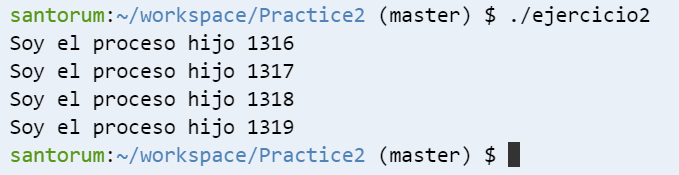
\includegraphics[scale=1.2]{ej2.PNG}
\end{center}


\section{Ejercicio 4}
Continuamos comentando el ejercicio 4, el segundo ejercicio a realizar. Este ya tiene un poco de complijidad ya que entran nuevas funciones con las cuales nunca hemos trabajado.\\\\
Su funcionalidad consiste en que el proceso padre crea un proceso hijo que realizará un trabajo (imprimir “Soy [PID] y estoy trabajando”). Pasado un tiempo, solicitará al padre que le releve un nuevo proceso hijo. El padre creará un nuevo proceso hijo y será, este nuevo proceso hijo, el encargado de avisar al hijo anterior de que ya puede terminar. Una vez avisado, el nuevo hijo empezará a trabajar de las misma manera.\\\\
Utilizaremos dos tipos de señales, \textbf{SIGTERM}, que será utilizada por cada proceso hijo para avisar al anterior hijo para que finalice (menos el último proceso hijo que será avisado por el padre). Además, también necesitaremos la señal \textbf{SIGUSR1} a la que le cambiaremos el manejador por defecto para que simplemente no ignore la señal y despertar al proceso padre de la función \texttt{pause()}.\\\\
Mostramos a continuación la salida de este ejercicio con número de procesos hijos igual a tres:
\begin{center}
	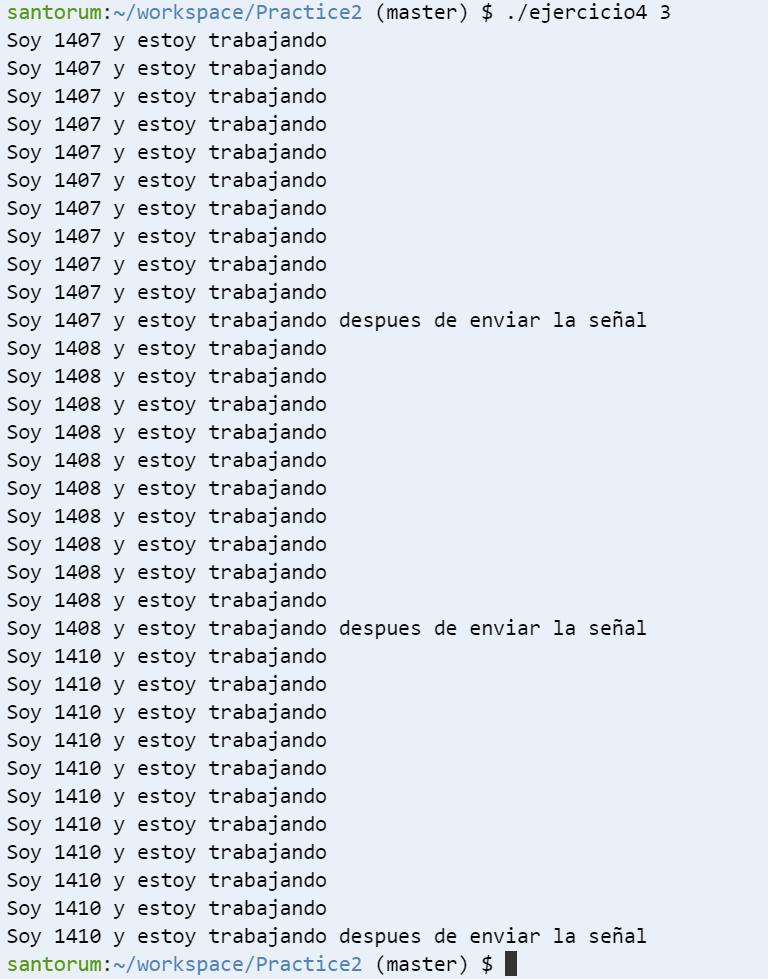
\includegraphics[scale=0.9]{ej4.PNG}
\end{center}
Poco que comentar esta salida. Los procesos hijos realizan su trabajo: imprimir 10 veces ese mensaje, y después envía la señal al padre para que lo releven. \\ Hemos añadido nosotros por nuestra cuenta una instrucción que consiste en mostrar por pantalla "Soy [PID] y estoy trabajando despues de enviar la señal" para informarnos de cuanto tiene que esperar el proceso hijo desde que envía la señal al padre, hasta que el nuevo proceso hijo le envía la señal de finalización. Vemos que solo tiene tiempo a imprimir una intrucción.\\\\
Comentar que el enunciado no aclara un detalle: pone que "Pasado un tiempo de 10 segundos (tras imprimir 10 veces el mensaje)..." lo cual no queda claro si hay que esperar adicionalmente 10 segundos después de todas las impresiones, o por el contrario, ya cuenta el tiempo usado para mostrar por pantalla los mensajes.\\ Hemos optado por usar la primera variante, esperar 10 segundos \textbf{después de todas} las impresiones. 

\section{Ejercicio 6-A}
Avanzamos hasta el siguiente ejercicio entregable, el ejercicio 6a. Se pide modificar el código proporcionado para que un proceso hijo, después de ser creado, establezca una alarma de 40 segundos. A continuación comenzará a ejecutar un bucle indefinidamente haciendo principalmente tres acciones: bloquear las señales \textbf{SIGALRM}, \textbf{SIGUSR1} y \textbf{SIGUSR2}, imprimir por pantalla los número 0, 1, ..., 4, y por último, desbloquear las señales \textbf{SIGALRM} y \textbf{SIGUSR1}, durmiendo antes de comenzar el bucle de nuevo durante 3 segundos.\\\\
El objetivo de bloquear las señales y después desbloquearlas es simple: impedir que finalice la ejecución del proceso cuando está realizando el trabajo, la impresión de números. Entonces, si la señal de alarma llega cuando está bloqueada \textbf{SIGALRM}, está esperará a que se desbloquee y el proceso finalizará normalmente.\\\\
La salida de este ejercicio es la que se muestra a continuación:
\begin{center}
	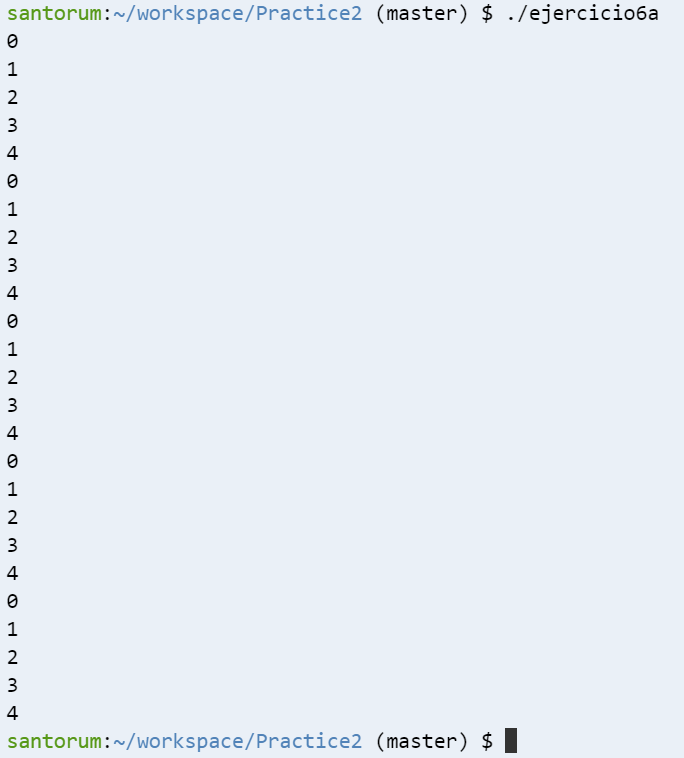
\includegraphics[scale=0.9]{ej6a.PNG}
\end{center}
Como la alarma está programada para 40 segundos, y el proceso hijo imprime 5 números en un intervalo de 5 segundos más una espera de tres, el proceso tiene tiempo para imprimir 5 veces el conjunto de números, tal y como se muestra en la salida.\\ Como se ha comentado anteriormente, si el proceso hijo reciviese la señal de alarma cuando esta está bloqueada, esta pasaría a estar en espera a que este desbloqueada y el proceso responda a ella, por lo que nunca el proceso va a acabar en mitad del trabajo de impresión.
\newpage


\section{Ejercicio 6-B}
Ahora explicamos la segunda parte del ejercicio 6, el apartado b. En este apartado el proceso principal (padre) crea un proceso hijo que realiza el mismo trabajo que el que realizaba en el apartado a. El padre esperará 40 segundos para a continuación enviar la señal \textbf{SIGTERM} para que el proceso hijo imprima "Soy [PID] y he recibido la señal SIGTERM" y finalice. Este procedimiento lo implementamos en un nuevo manejador distinto al de por defecto de la señal SIGTERM, por lo que necesitamos la ayuda de la función \texttt{signal(...)}.
\\Abajo mostramos la salida del programa comentado:
\begin{center}
	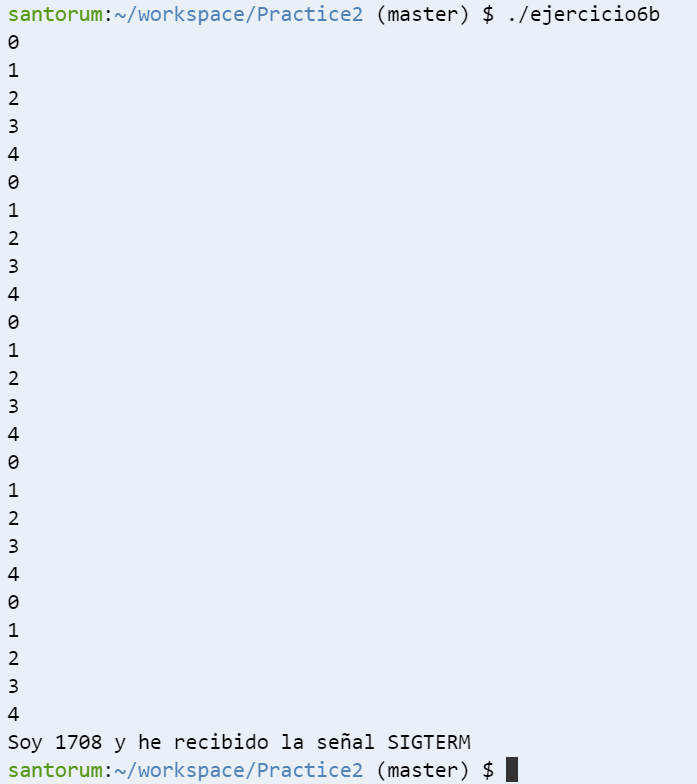
\includegraphics[scale=0.9]{ej6b_1.PNG}
\end{center}
Podemos ver que el proceso hijo ha hecho la función requerida, y cuando han pasado 40 segundos el proceso padre le envía la señal para que actúe como requería el enunciado.\\\\
Es importante comentar que cuando el proceso padre acaba la espera de 40 segundos y envía la señal de finalización al hijo, este justo acaba de imprimir el último número del turno. No obstante, a diferencia del ejercicio 6a, si la recibiese en otro momento, \textbf{interrupiría su ejecución y antendería la señal} ya que esta \textbf{ es la única que no está bloqueada}.\\
Modificando el tiempo de espera podemos apreciar esto. Aquí mostramos la salida solo cambiando el valor de la función \texttt{sleep()}:
\begin{center}
	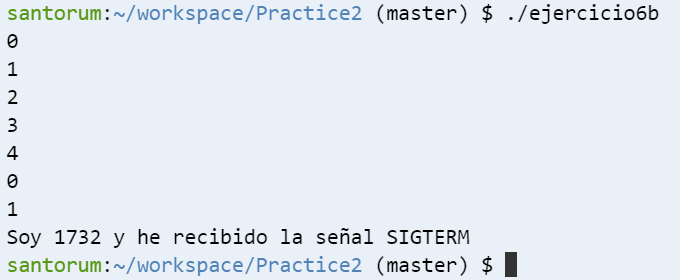
\includegraphics[scale=0.9]{ej6b_2.PNG}
\end{center}


\section{Biblioteca de Semaforos}
Llegamos al ejercicio donde tenemos que implementar la biblioteca de semaforos. Esta biblioteca, aparte de un gran ejercicio didáctico, si la logramos implementar correctamente nos servirá (ella o una pequeña modificación) enormemente en el futuro.\\\\
En primer lugar necesitamos indicar que las \textbf{cabeceras de las funciones aportadas por la documentación de la práctica no siguen la guía de estilo estándar de C} exigidas para las prácticas. Hemos hecho las funciones tal y como se indican en sus cabeceras, pero queremos dejar claro que tenemos la guía de estilo en cuenta.\\\\
Por otro lado, nos gustaría comentar un error que creemos (casi con seguridad) que tiene la especificación de las funciones UpMultiple\_Semaforo(...) y DownMultiple\_Semaforo(...). Se trata del parámetro de entrada size, que la documentación indica que es el tamaño del array de semáforos, pero nosotros lo hemos \textbf{adoptado como el tamaño del array de enteros *active}, ya que el tamaño del array de semaforos no es importante para semop(), pero en cambio el tamaño del array de enteros sí que es muy importante, tanto para la inicialización de la estructura sembuf, como para la funcion semop. Creemos que es una errata de la documentación.\\\\
Subrayar que las funciones, cuando devuelven ERROR, también imprimen por pantalla un mensaje explicativo de cual pudo haber sido el error. Esto es de gran utilidad para \emph{debuggear} en casos de fallo.\\\\
Aparte de esto, tenemos poco que comentar en cuanto a este ejercicio ya que no tenemos una forma rápida de comprobar si está bien implementado y la implementación se basa en estudiar el \texttt{man} de linux junto con los ejemplos de la documentación. Para ello utilizaremos el próximo ejercicio, que es bastante completo.\\\\


\section{Ejercicio 9}
Llegamos al último ejercicio de la práctica 2. No se puede decir que haya sido \emph{coser y cantar}, de hecho, el apartado de decisiones de diseño, dificultades encontradas y posibles futuras mejores es de un tamaño bastante importante.\\\\
Lo primero de todo, vamos a comentar poco a poco el fichero fuente 'ejercicio9.c' debido a que no tiene una envergadura adecuada para ser analizado si uno no ha participado en el desarrollo del mismo. Para ello se han incluido grandes cantidades de comentarios (en contra de la guía de estilo estándar de C, pero a favor de las peticiones de las documentaciones de las prácticas).\\\\
En primer lugar ya sabemos lo que toca, comprobación de errores de entrada: el número de argumentos tiene que ser igual a dos, el nombre y el número de cajeros del programa. Además, se incluye una función auxiliar implementada por nosotros 'is\_valid\_integer(char*)' que tiene el objetico de comprobar que realmente el segundo argumento es un entero.\\\\
Lo siguiente que hacemos es crear e inicializar los semáforos del programa: creamos  un array de $n+1$ semáforos, siendo $n$ el número de cajeros. Para esto nos valemos de las funciones de la biblioteca de semáforos. Subrayar una decisión de código: la \textbf{key} para la creación de semáforos (la cual será proporcionada a la función ftok(PATH, KEY)), es escogida aleatoriamente entre $MIN\_KEY=100$ y $MAX\_KEY=99999$ para reducir posibles errores (quizá el semáforo ya está creado, lo cual es mejor evitar) y hacer el sistema más robusto y portable a diferentes SSOO.\\ Utilizaremos los semáforos de índices $(1, 2, ..., n)$ para los ficheros que simularán las cajas de los cajeros y el semáforo de índice igual a $cero$ será el encargado de proteger el fichero de texto auxiliar para la comunicación de los procesos hijos con el padre. Todos los semáforos se inicializan a uno.\\\\
A continuación, creamos una máscara de señales con todas menos SIGUSR1 (utilizada por los hijos, cajeros, para avisar al padre de que retire dinero de su caja) y SIGINT, por si necesitamos utilizar ctrl+C. Esta máscara es activada de inmediato, siendo heredada en el futuro por los procesos hijos, y dejará de tener efecto al finalizar el programa (el S.O. se encargará de eso por nosotros).\\\\
Es en este momento cuando creamos $n$ = numero de cajeros = numero de ficheros de texto de clientes. Cada fichero de clientes le corresponderá a un cajero y tendrá una longitud de 50 transacciones. El coste de las transacciones es determiando aleatoriamente entre 0 y 300 tal y como indica en la documentación.\\\\
Ahora se crea el fichero de comunicación entre cajeros y gerente (hijos y padre), se asigna el nuevo manejador de SIGUSR1 y se crean los $n$ procesos hijos que simularán los cajeros.\\\\
A partir de este momento es cuando empieza "lo divertido" o mejor dicho, lo complicado. Por un lado, los procesos hijos usarán las funciones \textbf{nombre\_transaccion(int i)} y \textbf{nombre\_cajero(int i)}, que reciben el id (no el PID, el id del cajero) y devuelven el fichero de clientes(compras) y el fichero donde llevarán la contabilidad de la caja respectivamente. Gracias a ellas agilizarán la obtención de los nombres de archivos.\\\\
De seguido, cada cajero leerá de su archivo de clientes correspondiente (sin necesidad de semáforo porque nadie, además de ellos, intenta usar ese fichero) el valor de la transacción para a continuación, \textbf{bajando su semáforo de fichero}, actualizar la contabilidad de su caja, y \textbf{subir de nuevo el semáforo de caja}. Una vez termiando con esta secuencia de instrucciones, el cajero comprobará la cantidad actualizada de su caja, y si esta supera los $1000$ euros, \textbf{levantará el semáforo del fichero de cola de señales}, para introducir su id junto con una palabra indicadora de la acción a realizar, \emph{filled} para pedir que el padre le quite $900$ euros y se los lleve a la cuenta global, o \emph{fin} que indica que el cajero ha terminado de procesar ya las 50 transacciones de clientes. Una vez escrito esto en el fichero de cola, se enviará una señal SIGUSR1 al padre para despertarlo y el cajero \textbf{levantará el semáforo del fichero de la cola} para poder continuar trabajando, no sin antes realizar una espera de tiempo aleatorio entre uno y cinco segundos, que simula el tiempo de atención a un cliente real.\\\\
Mientras todo esto pasa, el proceso padre entrará en un bucle mientras el número de cajeros finalizados sea menor que el número de cajeros totales. Dentro de este bucle se pondrá a dormir usando la función \textbf{sigsuspend(\&set)} esperando a que algunos de los cajeros lo reclame.\\\\
Una vez que sea despertado, el proceso padre (gerente) \textbf{bajará el semáforo del fichero de cola de señales} para leer el id del cajero que lo llama, junto con la acción a realizar. Somos conscientes que una variante de este método sería que los cajeros enviaran dos señales diferentes (por ejemplo, SIGUSR1 y SIGUSR2), una solicitando que el padre les retire $900$ euros (manejador de SIGUSR1) y la otra solicitando que le vacíe la caja porque ha finalizado (manejador de SIGUSR2). No se ha adoptado este método por simplificidad del código, ya que seguir esta línea implicaría crear un manejador nuevo, nuevas variables globales, y una máscara diferente; pero este es la cruz a la que se tiene que someter un programador: memoria vs eficiencia, no siempre las dos son mejorables al mismo tiempo.\\\\
Siguiendo con la explicación del funcionamiento, una vez que el proceso padre sepa que tiene que hacer, \textbf{bajará el semáforo de la caja correspondiente}, haciendo los cambios pertinentes y volviendo a \textbf{levantar el semáforo de la caja} al momento. Una vez terminado con el archivo de cola de señales, el padre lo vaciará para poder saber en el futuro, cuales son las señales no leídas (lógicamente, las que no han sido borradas aún), y finalmente, \textbf{levantará el semáforo del semáforo de cola}.\\\\
Es importante en este momento explicar el funcionamiento de la única variable global utilizada: \textbf{flag}. Su misión es encargarse de informarle al padre \textbf{si una señal SIGUSR1 ha llegado antes de que este se ponga de nuevo a dormir}. Tenemos que tener en cuenta que desde que el padre levanta el semáforo de caja, hasta que se pone de nuevo en el estado de \emph{sleeping}, pasa un tiempo insignificante, solo dos comprobaciones lógicas. En cambio, cualquier cajero tendría que abrir un fichero, leerlo, hacer alguna operación, escribir en el fichero, cerrar el fichero y enviarle la señal al padre en el tiempo que este hace dos míseras comprobaciones lógicas.\\ Esto parece de poca importancia en la práctica, pero en la teoría sabemos que no podemos \textbf{hacer suposiciones sobre el tiempo de ejecución de ningún proceso, por inverosímil que parezca}, que ahí que hagamos \textbf{sigsuspend(...)} si y solo si flag es igual a cero, lo que quiere decir que no hemos entrado en el manejador de SIGUSR1, que pone flag a 1.\\\\
Una vez que todos los cajeros hayan finalizado, el proceso padre \textbf{eliminará los semáforos} y hará el recuento total de las cajas, utilizando la función \textbf{final\_check(int n, int total)}, que lo que hace es sumas todas las transacciones de los ficheros de clientes y comparar el resultado con el obtenido por el gerente (proceso padre) después de procesar todas las señales.\\\\
Antes de dar paso a un ejemplo de salida de este programa, tenemos que hacer un par de aclaraciones y/o comentarios.\\ En primer lugar, a simple vista parece que el 'ejercicio9' es de un tamaño significativo, pero si le quitamos las líneas de comentarios y las de comprobaciones de errores (que no son pocas precisamente, es lo que tiene trabajar de una forma segura y robusta), nos quedamos con un código "simple". Lo único que se hace es que varios procesos utilicen ficheros de texto, pero esto nos sirve para comprobar el correcto funcionamiento de nuestros semáforos, además de servir de un ejercicio didáctico enorme.\\\\
Por último, nos gustaría subrayar una decisión de diseño importante. A la hora de subir o bajar semáforos utilizamos \textbf{espera activa}, que es una técnica donde un proceso verifica repetidamente una condición, en este caso lo normal es no REPETIR DICHA VERIFICACIÓN, pero puede darse el caso que no se pueda hacer la bajada/subida de semáforo por cualquier razón del sistema. Esta es la razón por la que se realiza una espera activa. Comentar que nunca hemos abandonado la posibilidad de que realmente suceda un error con los semáforos, por lo que hemos añadido una comprobación de intentos máximos de espera activa (directamente proporcional al número de cajeros). Si se supera el número de intentos máximo, se considera que el semáforo ha fallado por completo, y cortamos la ejecución del programa de inmediato, liberando todos los recursos y comunicándoselo al usuario por pantalla.

Por fin, ahora vamos ha mostrar una salida de este programa:
\begin{center}
	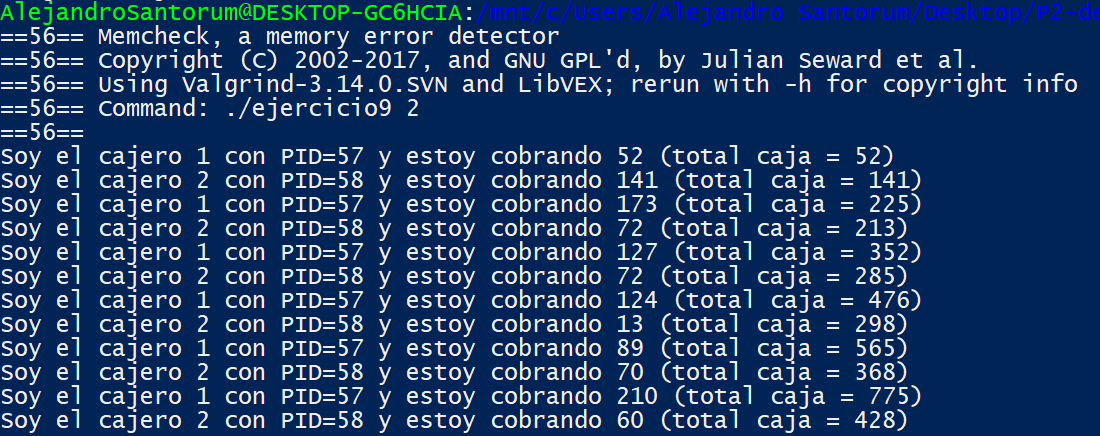
\includegraphics[scale=1]{ej9_1.PNG}
\end{center}
La salida es más amplia que lo que mostramos ya que se ha incluído una cantidad considerable de impresiones por pantalla para darnos información del desarrollo de los cajeros. Otra razón de peso para mostrar una salida así de poblada, es para no inquietarnos esperando a que el programa acabe, ya que la terminal estará parpadeando durante una media de $\frac{2.5*60*n}{60}$ minutos, que para solo dos procesos son aproximadamente $4$ minutos, lo cual hace pensar muchas veces que el programa \emph{se ha colgado}. Si no desea esta salida, puede simplemente comentar 1 línea de código.\\\\
\newpage
Ahora mostramos la parte final de la salida del programa, omitiendo el resto de "Soy el cajero [ID] con PID=[PID] y estoy cobrando [precio\_compra] (total caja = [cantidad\_caja\_actual])".
\begin{center}
	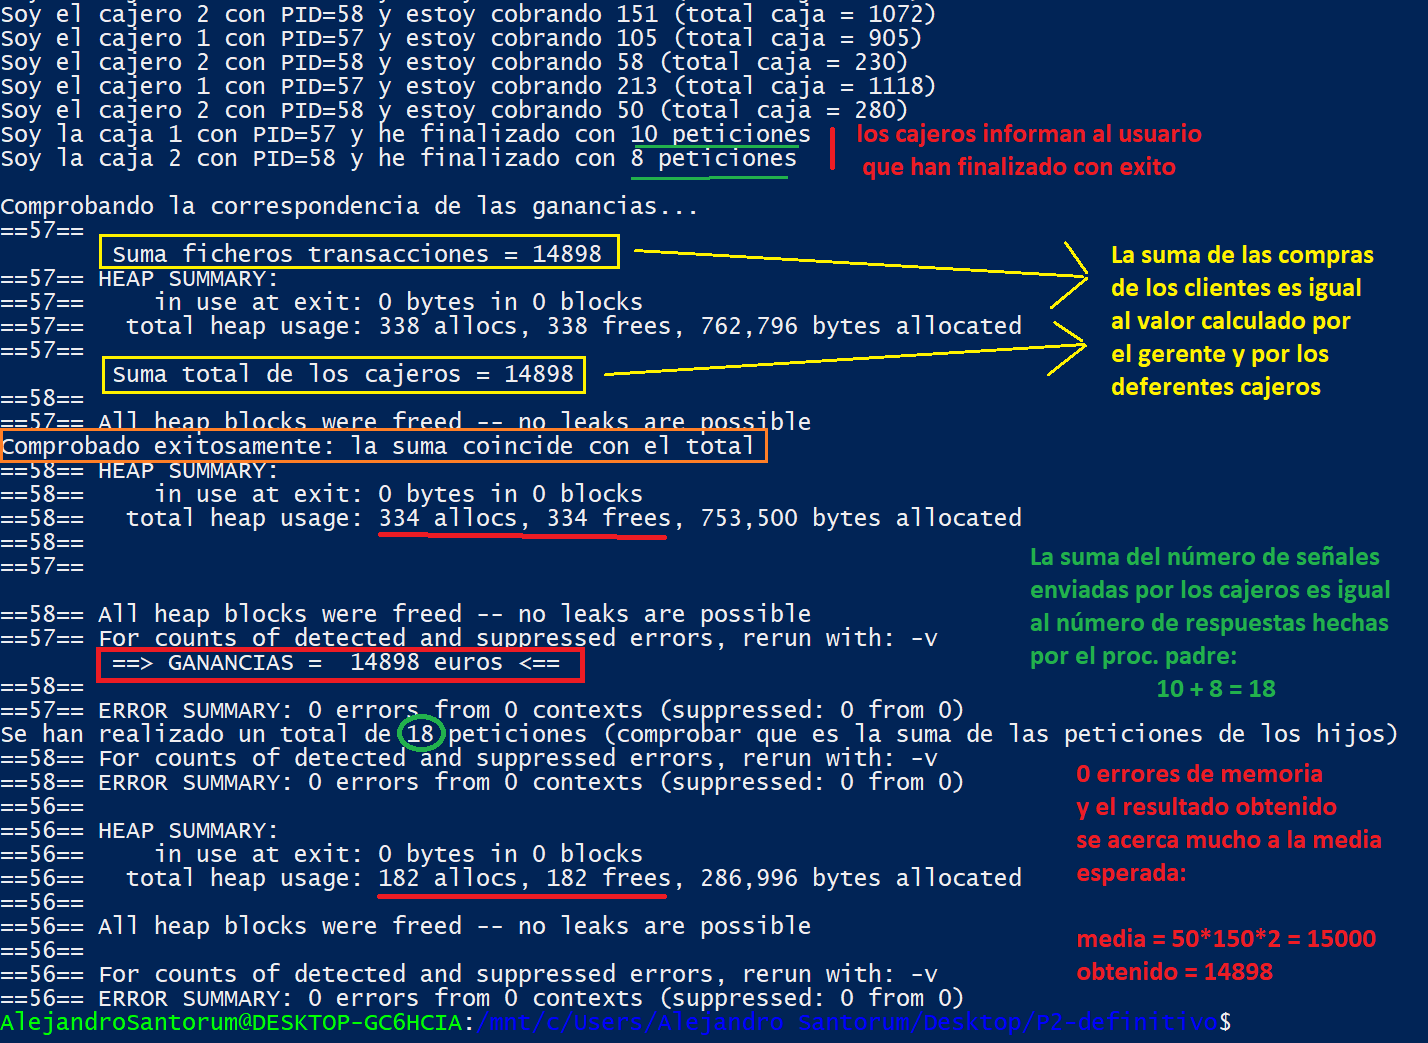
\includegraphics[scale=1]{ej9_2.PNG}
\end{center}
Invitamos a probar diferentes numeros de cajeros, pero siempre teniendo en cuenta el tiempo que puede llegar a tardar la demora: $t_{M} = \frac{2.5*60*n}{60}$ ($t_{M} = tiempoMedio$).\\\\
Una vez que se termine de probar/ejecutar el programa las veces que se quiera, recomendamos ejecutar \textbf{make clean} para limpiar los archivos binarios compilados, y \textbf{make text} para eliminar todos los ficheros de texto de la carpeta \texttt{txtfiles}. Estos ficheros, si el programa se ha ejecutado con exito, deberán estar en el siguiente estado: el fichero de cola de señales estará vacío (el proceso padre ha leído todas las señales), los archivos que simulan las cajas ($cajero_i$) deberán tener escrito el número cero, lo que quiere decir que todo su dinero ha sido retirado satisfactoriamente. Por último, en los ficheros de clientes ($clientesCaja_i$) estarán las transacciones de los clientes creadas en la última ejecución del programa. Hemos dejado los ficheros de texto sin eliminarlos para hacer cualquier comprobación de error.

\section{Conclusión y comentarios finales}
Señalar que en los primeros cuatro ejercicios no se ha incluido el informe de \emph{Valgrind} pero sabemos con certeza que no tienen ningún error de memoria.\\\\
Ahora sí, una vez finalizada la práctica tenemos que echar una mirada atrás y ver todo lo que hemos aprendido. Hemos tomado contacto con las señales entre procesos y con los semáforos. Han sido 2-3 semanas intensas con una gran cantidad de funciones nuevas que jamás habíamos utilizado, y que ahora nos permitirán realizar programas mucho más exigentes.\\\\
Nos llevamos un sabor agridulce, ya que el ejercicio9, el destinado a utilizar semáforos, era ciertamente enrevesando, ya que nos obligada a comunicar de alguna forma dos procesos al mismo tiempo que utilizábamos semáforos y envíabamos señales. Es una pena que tengamos que realizar ciertos "apaños" rudimentarios para poder coordinar los procesos, pero es lo que 
tenemos a mano actualmente, hasta que veamos los temas futuros.\\\\
Error tras error se ha ido aprendiendo y esperamos haber hecho una buena práctica.
\end{document}
	